\documentclass[10pt]{beamer}
\usepackage[UTF8]{ctex}
\usepackage{outlines}
\usepackage{hyperref}
\ifx\pdfoutput\undefined
% we are running LaTeX, not pdflatex
\usepackage{graphicx}
\else
% we are running pdflatex, so convert .eps files to .pdf
\usepackage{graphicx}
\usepackage{epstopdf}
\fi

%--------------------------------------------------------
% NOTE: 1) This is an UNOFFICIAL LaTeX beamer style for 
%           Beihang University.
%       2) This is not exactly a beamer style, rather
%           it contains two LaTeX files to be inserted 
%           in the slides' source file.
%       3) These files are based on Edward Hartley's work
%   <http://www-control.eng.cam.ac.uk/Main/EdwardHartley>
%       4) Complaints or suggestions are always welcome.
%
% Xiaoke Yang (das.xiaoke@hotmail.com)
% Wed 15 Jun 11:02:17 CST 2016
%--------------------------------------------------------


%--------------------------------------------------------
% Set up the Beihang University Colours for use with
% xcolor
%--------------------------------------------------------

% Blue palette
\definecolor{coreBlue}{rgb}{0.02 0.30588 0.64706} %#254aa5


%--------------------------------------------------------
% NOTE: 1) This is an UNOFFICIAL LaTeX beamer style for 
%           Beihang University.
%       2) This is not exactly a beamer style, rather
%           it contains two LaTeX files to be inserted 
%           in the slides' source file.
%       3) These files are based on Edward Hartley's work
%   <http://www-control.eng.cam.ac.uk/Main/EdwardHartley>
%       4) Complaints or suggestions are always welcome.
%
% Xiaoke Yang (das.xiaoke@hotmail.com)
% Wed 15 Jun 11:02:17 CST 2016
%--------------------------------------------------------

%--------------------------------------------------------
% Require tikz to do some text positioning
%--------------------------------------------------------
\usepackage{tikz}

%--------------------------------------------------------
% Use Helvetica rather than Computer Modern Sans Serif
% Comment this out if you prefer Computer Modern
%\usepackage{times}
%--------------------------------------------------------
%\usepackage{helvet}

%--------------------------------------------------------
% If you wish to use Arial, and have the winfonts package
% correctly installed uncomment the following to make the
% default sans serif font Arial
%--------------------------------------------------------
%\usepackage{winfonts}
%\usepackage[T1]{fontenc}
%\renewcommand{\sfdefault}{arial}
%--------------------------------------------------------

%--------------------------------------------------------
% Get rid of the navigation bar 
%--------------------------------------------------------
\beamertemplatenavigationsymbolsempty

%--------------------------------------------------------
% Set the files corresponding to the University crests
% here
%--------------------------------------------------------
% Crest with blue text
\newcommand{\beihangcrestblack}{beihangbeamerstyle/beihang-pantone}

% Crest with white text
\newcommand{\beihangcrestwhite}{beihangbeamerstyle/beihang-rev-pantone}
%--------------------------------------------------------

%--------------------------------------------------------
% Define how the page counter will be displayed on slides
%--------------------------------------------------------
\newcommand{\footlinepagecounter}%
	{\insertframenumber{}/\inserttotalframenumber}
%--------------------------------------------------------

%--------------------------------------------------------
% Set up some lengths
%--------------------------------------------------------
% A paper width for the footline
\newlength{\halfpaperwidth}

% The left margin
\newlength{\headingleftmargin}
% Paper width minus margins
\newlength{\headingwidthminusmargins}
% Height of the heading block
\newlength{\headingheight}
% Height of the footer block
\newlength{\footerheight}

% The height for the titlepageheader in the title page
\newlength{\titlepageheaderheight}
% The height for the footer in the title page
\newlength{\titlepagefooterheight}
% The height for the main title block
\newlength{\titlepagemaintitleblockheight}
% The height for the subtitle block
\newlength{\titlepagesubtitleblockheight}
% The height for the name and date block
\newlength{\titlepagenamedateblockheight}
% The height for the institution block
%\newlength{\titlepageinstitutionheight}

% The lengths for spacing between name and date
\newlength{\titlepagespaceundername}
\newlength{\titlepagespaceunderdate}

% The length for the light blue thin bar


\setlength{\headingleftmargin}{0.05573\paperwidth}
\setlength{\headingwidthminusmargins}{\paperwidth}
\addtolength{\headingwidthminusmargins}{-\headingleftmargin}
\setlength{\headingheight}{0.1459\paperheight}
\setlength{\footerheight}{0.09017\paperheight}

\setlength{\titlepageheaderheight}{0.2361\paperheight}
\setlength{\titlepagefooterheight}{0.1459\paperheight}
\setlength{\titlepagemaintitleblockheight}{0.2361\paperheight}
\setlength{\titlepagesubtitleblockheight}{0.1459\paperheight}
\setlength{\titlepagenamedateblockheight}{0.2361\paperheight}
%\setlength{\titlepageinstitutionheight}{0.95cm}

\setlength{\titlepagespaceundername}{16pt}
\setlength{\titlepagespaceunderdate}{8pt}

%--------------------------------------------------------

%--------------------------------------------------------
% Set up the Beihang University blue scheme for use
% with beamer
%--------------------------------------------------------

% Define colour names
\setbeamercolor{coreBlue}{bg=coreBlue, fg=white}

% Set element colours
\setbeamercolor{subtitle}{fg=white}
\setbeamercolor{titlepageheader}{bg=white,fg=black}
\setbeamercolor{titlepagefooter}{bg=white,fg=black}
\setbeamercolor{block title}{bg=white, fg=coreBlue}
\setbeamercolor{structure}{bg=white, fg=coreBlue}
% \setbeamercolor{alerted text}{fg=darkOrange}


%--------------------------------------------------------
% Set font sizes
%--------------------------------------------------------
\setbeamerfont{frametitle}{size=\large,series=\bfseries}
\setbeamerfont{title}{size=\large,series=\bfseries}
\setbeamerfont{author}{size=\normalsize}
\setbeamerfont{date}{size=\scriptsize}
\setbeamerfont{subtitle}{size=\footnotesize,series=\bfseries}
\setbeamerfont{block title}{size=\normalsize,series=\bfseries}
\setbeamerfont{structure}{size=\normalsize,series=\bfseries}

\setbeamertemplate{itemize item}{\scriptsize\raise1.25pt\hbox{\textbullet}}
\setbeamertemplate{itemize subitem}{\scriptsize\raise1.25pt\hbox{\textbullet}}
\setbeamertemplate{itemize subsubitem}{\scriptsize\raise1.25pt\hbox{\textbullet}}


%-----------------------------------------------------
% Define frame title drawing
%-----------------------------------------------------
\setbeamertemplate{frametitle}
{%
  \nointerlineskip
  \begin{beamercolorbox}[wd=\paperwidth,leftskip=\headingleftmargin]{coreBlue}
    \vskip1pt%
    \tikz{\node[minimum height=\headingheight, inner sep=0cm, text width= \headingwidthminusmargins, text badly ragged]{\usebeamerfont{frametitle}\insertframetitle\\\normalsize\it\insertframesubtitle};}
  \end{beamercolorbox}%
}

%-----------------------------------------------------
% Define footline drawing
%-----------------------------------------------------
\setbeamertemplate{footline}
{%
 \setlength{\halfpaperwidth}{0.5\paperwidth}
 \addtolength{\halfpaperwidth}{1pt}
 \leavevmode
 \begin{beamercolorbox}[sep=0pt,wd=\halfpaperwidth, leftskip=\headingleftmargin,right]{coreBlue}
 \tikz{\node[minimum height=\footerheight, inner sep=0cm]{\footlinepagecounter};}%
 \end{beamercolorbox}
 \hskip-1.5pt%
 \begin{beamercolorbox}[sep=0pt,wd=\halfpaperwidth, leftskip=\headingleftmargin, right,rightskip=\headingleftmargin]{coreBlue}
 \tikz{\node[minimum height=\footerheight, inner sep=0cm]{\includegraphics[width=0.25\paperwidth]{\beihangcrestwhite}};}%
 \end{beamercolorbox}%
}


%-----------------------------------------------------
% Define BEIHANG title page
%-----------------------------------------------------
\setbeamertemplate{title page}
{%
\begin{beamercolorbox}[sep=0cm,right,wd=\paperwidth,ht=\titlepageheaderheight,rightskip=\headingleftmargin]{titlepageheader}
\includegraphics[width=0.3820\paperwidth]{\beihangcrestblack}
\vskip0.2361\titlepageheaderheight
\end{beamercolorbox}
\begin{beamercolorbox}[left,leftskip=\headingleftmargin,wd=\paperwidth,ht=\titlepagemaintitleblockheight]{coreBlue}
\tikz{\node[inner sep=0cm, text width=\paperwidth, minimum height=\titlepagemaintitleblockheight,text badly ragged]{\usebeamerfont{title}\inserttitle};}%
\end{beamercolorbox}%
\nointerlineskip%
\vskip-1pt%
\begin{beamercolorbox}[left,leftskip=\headingleftmargin,wd=\paperwidth,ht=\titlepagesubtitleblockheight]{coreBlue}
\tikz{\node[inner sep=0cm, text width=\paperwidth, minimum height=\titlepagesubtitleblockheight, text badly ragged]{\usebeamerfont{subtitle}\usebeamercolor[fg]{subtitle}\insertsubtitle};}%
\end{beamercolorbox}%
\nointerlineskip%
\vskip-1pt%
\begin{beamercolorbox}[left,leftskip=\headingleftmargin,wd=\paperwidth,ht=\titlepagenamedateblockheight]{coreBlue}
      \usebeamerfont{author}\insertauthor\\
      \vskip\titlepagespaceundername%
      \usebeamerfont{date}\insertdate
      \vskip\titlepagespaceunderdate%
    \end{beamercolorbox}%
\begin{beamercolorbox}[left,leftskip=\headingleftmargin,wd=\paperwidth,ht=\titlepagefooterheight]{titlepagefooter}
\end{beamercolorbox}
}


\title{计算机世界入门}
\author{张博涵\\
北京航空航天大学经济管理学院 (\texttt{zhangbohan@buaa.edu.cn})}
\date{\today}


\begin{document}
%----------------------------------------------------------------------
% Title frame
\begin{frame}[plain]
\maketitle
\end{frame}

%----------------------------------------------------------------------
% Outline frame
% PLEASE RUN pdflatex TWICE 
\begin{frame}
\frametitle{Outline}
\tableofcontents
\end{frame}
%%=====================================================================
% Section I
\section{引言}
%----------------------------------------------------------------------
% Content frame
\begin{frame}
\frametitle{编程有哪些应用?}
\framesubtitle{大应用}
\begin{block}{操纵硬件}
    操作系统、智能机器人、嵌入式设备、智能家居
\end{block}
\begin{block}{信息的收集、处理、储存、分发}
    互联网、应用程序、数据库、健康码、区块链
\end{block}

\begin{block}{模拟、分析与认知世界}
    大气模拟、导弹弹道模拟、游戏、VR、人工智能
\end{block}
\end{frame}

\begin{frame}
\frametitle{编程有哪些应用?}
\framesubtitle{小应用}
    \begin{outline}
        \1 家庭服务器 
            \2 \url{https://nextcloud.ponez.me:444/}
            \2 \url{https://nextcloud.ponez.me:445/}
            \2 树莓派、智能家居
        \1 爬虫与\href{https://zh.m.wikipedia.org/zh/RSS}{RSS}
            \2 \href{https://docs.rsshub.app/}{RSSHub}
        \1 IFTTT与自动化
            \2 IFTTT: If this then that
            \2 定时任务
    \end{outline}
\end{frame}

%%=====================================================================
% Section II
\section{硬件与操作系统}
%----------------------------------------------------------------------

\begin{frame}
\frametitle{现代计算机的起源}
\framesubtitle{图灵机}
\begin{itemize}
    \item 1936年由英国数学家艾伦·图灵提出,是一种“计算模型”
    \item 可以表达任何有限逻辑数学过程,例如$1+1$
\end{itemize}
\begin{figure}
    \centering
    
\includegraphics[width=0.5\textwidth]{figures/tuling.png}    
\end{figure}

\begin{block}{通用图灵机:现代电子计算机的计算模型}
    \begin{itemize}
        \item 将图灵机进行编码$<M>$
        \item 当计算核心遇到编码$<M>$时,模拟图灵机$<M>$的运行
        \item 这些被编码的图灵机称为“程序”
    \end{itemize}
\end{block}
现代计算机采用0-1二进制对数据和程序进行编码

\end{frame}

\begin{frame}
\frametitle{现代计算机的起源}
\framesubtitle{冯·诺伊曼结构}

\begin{itemize}
    \item 冯·诺伊曼结构是实现通用图灵机的一种计算设备
    \item 存储程序计算机
    \item 执行步骤:提取、解码、执行和写回
\end{itemize}

\begin{figure}
    \centering
    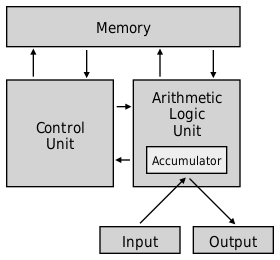
\includegraphics[width=0.5\textwidth]{figures/Von_Neumann_architecture..png}
\end{figure}

\end{frame}

\begin{frame}
\frametitle{通用计算设备}
\framesubtitle{以PC(personal computer)为例}

\begin{block}{一般PC的组成}
    \begin{outline}
        \1 CPU:中央处理器,核心的计算单元
        \1 GPU:图形处理器,图形渲染,完全的并行计算
        \1 内存:临时的数据
        \1 硬盘:长期数据存储
        \1 主板:连接各种设备
    \end{outline}
\end{block}

\end{frame}

\begin{frame}
\frametitle{PC与操作系统}
\begin{block}{操作系统}
    \begin{itemize}
        \item 操作系统是人与计算机硬件进行交互的中介。在大多数情况下,只要具有以上的硬件,操作系统可以安装在不同型号的硬件上(“兼容”),但也有些时候它们是绑定的。
        \item PC: Linux、MacOS、Windows
        \item 智能手机:iOS、Android
        \item 其他智能设备
    \end{itemize}
\end{block}

\begin{columns}
    \begin{column}{0.7\textwidth}
        \begin{block}{主要芯片厂商}
            \begin{itemize}
                \item Intel:酷睿系列CPU i3 i5 i7 i9
                \item Apple:M1, M1 pro, M2
                \item AMD:锐龙系列CPU
                \item Nvidia:RTX系列GPU
            \end{itemize}
        \end{block}
    \end{column}
    \begin{column}{0.3\textwidth}
        \begin{block}{CPU架构}
            \begin{itemize}
                
                \item x86
                \item ARM
            \end{itemize}
        \end{block}
    \end{column}
\end{columns}

\end{frame}

\begin{frame}
    \frametitle{PC与操作系统}

        \begin{itemize}
            \item Windows与Linux系统的计算机大多可以自己组装,选择需要的CPU、GPU、内存、硬盘等型号并更换。
            \item MacOS系统由Apple开发,主要应用于自家的Mac电脑产品上,只能通过不正规的渠道安装在自己的硬件上。
        \end{itemize}
\end{frame}

\begin{frame}
\frametitle{Linux与开源}
\begin{figure}
    \centering
    
\includegraphics[width=0.1\textwidth]{figures/linux.jpeg}
\end{figure}

\begin{itemize}
    \item 自由和开放源代码的操作系统,社区驱动开发,任何人或组织可以在Linux内核的基础上修改源代码、开发自己的发行版,甚至基于此盈利。
    \item 世界上90\%以上的服务器以及世界500强超级计算机运行在Linux及其变体上,目前在个人电脑上的占有率也逐渐上升。
    \item Windows现在支持Linux内核
    \item 衍生版本:Ubuntu、Debian、CentOS、Deepin等
\end{itemize}
\end{frame}

\section{编程语言}


\begin{frame}
\frametitle{语言类型}

\begin{itemize}
    \item 机器语言:是电脑的CPU 或 GPU 可直接解读的程序,用二进制代码表示
    \item 汇编语言:汇编语言使用助记符(Mnemonics)来代替和表示特定低级机器语言的操作。
    \item 高级语言:以人类的日常语言为基础的编程语言,使用一般人易于接受的文字来表示,有较高的可读性,以方便对电脑认知较浅的人亦可以大概明白其内容,主要为英语。
    \item 现代程序的开发几乎都采用高级语言。
\end{itemize}
\end{frame}

\begin{frame}
\frametitle{现代的高级语言}

\begin{table}
    \centering
    \begin{tabular}{ccccc}
    C &  C++ & Python & Java & R \\
    
\includegraphics[width=0.1\textwidth]{figures/C.png} &
    
\includegraphics[width=0.1\textwidth]{figures/C++.png} & 
    
\includegraphics[width=0.1\textwidth]{figures/python.png} & 
\includegraphics[width=0.1\textwidth]{figures/java.png} &
    
\includegraphics[width=0.1\textwidth]{figures/R.png} \\
    Julia &  Go  & Rust & JavaScript & php \\
    
\includegraphics[width=0.1\textwidth]{figures/julia.png} &
    
\includegraphics[width=0.1\textwidth]{figures/go.png} & 
    
\includegraphics[width=0.1\textwidth]{figures/rust.png} & 
\includegraphics[width=0.1\textwidth]{figures/javascript.png} &
    
\includegraphics[width=0.1\textwidth]{figures/php.png}
    \end{tabular}
\end{table}

除了列出的之外,还有非常非常多。不同的编程语言有各自的特点和擅长的领域,例如C、C++、Rust主要用于系统编程、底层开发等方面;Julia优势在于科学计算方面;R主要用于数据分析与统计建模;Python在人工智能、数据分析、Web开发等方面都应用广泛。

\end{frame}

\section{编程相关软件和环境}

\begin{frame}
\frametitle{Shell}

\begin{itemize}
    \item Shell是操作系统中提供内核访问之服务的工具,是程序员与操作系统进行沟通的桥梁,狭义上来说就是所谓的“命令行界面” + 访问其他应用程序的脚本语言。
    \item 代表性的Shell有Windows下的cmd.exe, PowerShell,Linux及MacOS等类Unix系统下的bash, zsh等。
    \item 在Shell中可以编译和运行程序、操作和处理文件等等
    \item 参考课程:\url{https://missing-semester-cn.github.io/2020/course-shell/} 
\end{itemize}

课后作业一:阅读参考链接并安装Windows Subsystem for Linux


\end{frame}

\begin{frame}
\frametitle{认识文件}

\begin{itemize}
    \item 文件:\textbf{文件名}.\textbf{文件后缀}
    \item 文本文件:只有字符原生编码构成的二进制计算机文件,与富文本相比,其不包含字样样式的控制元素,能够被最简单的文本编辑器直接读取。编程时主要用到的存放源代码的文件。
    \item 富文本文件:docx、pptx, xlsx,需要特定的应用程序进行处理。
    \item 二进制文件:可执行程序,例如微信.exe
    \item 媒体文件:视频、图像等等
\end{itemize}


\end{frame}

\begin{frame}
\frametitle{文本编辑器、IDE}

这里的文本编辑器指用于处理纯文本文件的编辑器。

\begin{itemize}
    \item Windows下的记事本,功能过于简单
    \item Shell:vim、vi、emacs,过于复杂,不适用于新手
    \item 其他专门用于编程的文本编辑器:Visual Studio Code, Sublime Text, Atom等
\end{itemize}

\begin{block}{IDE:集成开发环境}
    将编程的所需要的各个步骤如代码的编辑、编译、测试、发布等集成到一起的辅助程序员的软件工具。
\end{block}

推荐:Visual Studio Code

\end{frame}


\begin{frame}
    \frametitle{练习}
    \begin{itemize}
        \item 安装 Visual Studio Code 以及 Python 并配置Python环境
        \item Hello World!
    \end{itemize}
    
\end{frame}


\begin{frame}
\frametitle{养成好的习惯}

\begin{itemize}
    \item 记笔记
    \item 查资料
    \item Keep your hands dirty!
\end{itemize}
\end{frame}

\begin{frame}
\frametitle{后续课程安排}
\begin{itemize}
    \item Python 入门
    \item 案例:爬虫
    \item 案例:图像压缩
    \item Git、Github与版本控制
    \item ...
\end{itemize}
\end{frame}

\end{document}


